\documentclass[11pt]{beamer}  
\usepackage{xeCJK}  
\usepackage{mathdots}  
\usepackage{graphicx}  
\usepackage{float}  
\usepackage{multirow}  
%\usepackage{cite}  
\usepackage{amsfonts, amsmath, mathrsfs, amsbsy, amssymb, dsfont,setspace}
\usepackage[square, comma, sort&compress, numbers]{natbib} 
%\usetheme{Warsaw}  
\usetheme{CambridgeUS}
\begin{document} 
\title{减弱墙体杂波的方法的相关整理}  
\author{黄臣}  
\date{\today}  
\frame{\titlepage}  
\begin{frame}
  \frametitle{Background}
  在穿墙雷达成像的整个环节中,我们面临的最大问题就是强烈的墙体反射杂波对墙后
  微弱目标的掩盖。以往的方法是在成像前,对接收到的信号进行背景扣除,用于去除
  来自天线的串扰和墙体反射。也就是从接收信号中减去没有目标存在时的回波数据,
  但是往往很难预先获取空场景时的回波数据\citep{Ahmad2015Wall}。
  \par 由于在雷达回波中,墙壁反射杂波是最强的组成部分,且墙体反射波在阵列孔径
  中具有不变性,\citep{Tivive2011An}指出可以通过对测量的数据矩阵应用奇异值分解,
  墙壁反射杂波占据低维子空间并且可以被与主要奇异值相关联的奇异向量捕获,从而完成了杂波抑制。

\end{frame}
\begin{frame}
  \frametitle{Background}
  考虑到傅里叶基被认为不适合表示墙壁杂波中的所有能量,
  因为它往往被用于表示点目标模型,而墙体是空间拓展目标,其电气参数又与频率
  有关,所以墙体回波不符合点目标模型\citep{Ahmad2015Wall}。所以可以
  使用基于离散长椭球体序列(DPSS)的字典来表示墙体回波,然后利用
  接收信号中的块稀疏特性,采用BOMP的方法来捕获信号\citep{Ahmad2015Wall}。这样做的好处是DPSS能够在给定的时间间隔内使能量集中最大化,
  所以DPSS可以很好地逼近墙体回波信号\citep{Slepian1978Prolate}\citep{Zhu2015Approximating}。
  \par 考虑所有天线都观测到了相同的墙和目标,可以联合所有的天线建模墙壁和回波
  和目标的回波来建立子空间模型,\citep{Davenport2011Compressive}则指出当DPSS长度为$2NW$时能在MSE意义上最近似表示原信号。由于使用DPSS表征墙壁回波的子空间,因此无需
  像\citep{Tivive2011An}一样需要全部数据,令后续的稀疏重建问题得到有效利用\citep{Zhu2016On}。
\end{frame}
\begin{frame}
  \frametitle{SVD-based Approach}
  使用奇异值分解在B-Scan矩阵上提取目标特征,一开始被用于探地雷达上。\citep{Chandra2008An}\citep{Verma2009Analysis}
  指出在TWRI的杂波消除中,目标信息往往聚于B-scan矩阵的第二特征分量附近,而杂波位于第一特征分量。
  \citep{Tivive2011An}则证明了目标反射并非只存在于B-scan矩阵的第二特征分量
  中,也可能跨越子空间,这取决于目标位置和数量。
\end{frame}
\begin{frame}
  \frametitle{SVD-based Approach}
  首先来自每个天线的接收信号可以表示为A-scan的形式:
  \begin{equation}
	{\boldsymbol s}_{n}(z)=\sum_{m=0}^{M-1}y(n, m)\exp(j2\pi f_{m}t)
  \end{equation}
  对每个A-scan值减去其平均值得到$\tilde{{\boldsymbol s}}_{n}$,联合所有单独的
  A-scan可以得到B-scan:
  \begin{equation}
	{\boldsymbol S}=[\tilde{{\boldsymbol s}}_{1},\tilde{{\boldsymbol s}}_{2}, \cdots,\tilde{{\boldsymbol s}}_{n}]
  \end{equation}
\end{frame}
\begin{frame}
  \frametitle{SVD-based Approach}
  对B-scan做奇异值分解,可以得到其特征分量的线性组合:
  \begin{equation}
	{\boldsymbol S}=\sum_{i=1}^{N}w_{i}({\boldsymbol u}_{i}{\boldsymbol v}_{i}^{T})=w_{1}{\boldsymbol E}_{1}+w_{2}{\boldsymbol E}_{2}+\cdots+w_{n}{\boldsymbol E}_{N}
  \end{equation}
  可以将特征分量划分为三个子空间:
  \begin{equation}
	{\boldsymbol E}=[{\boldsymbol E}_{1\rightarrow k}\vert {\boldsymbol E}_{k+1\rightarrow p}\vert {\boldsymbol E}_{p+1\rightarrow N}]
  \end{equation}
  根据模拟仿真可以确定前几个特征分量具有最大奇异值的为墙壁反射的子空间可以
  直接减去,剩余的组成新的B-scan矩阵,权值定义为:
  \begin{equation}
	w_{i}={1\over 1+({q-1\over \beta L})^{\alpha}} \qquad\qquad\forall\ q=1, \cdots, L 
  \end{equation}
\end{frame}
\begin{frame}
  \frametitle{DPSS Approach}
  DPSS能使给定频带内的能量集中最大化\citep{Slepian1978Prolate},对于给定的
  $W\; \in\; (0,\frac{1}{2})$和$N\;\in\;\mathbb{N}$,DPSS的前$2NW$项特征值
  趋近集中在$1$附近,剩余特征值趋近集中在$0$附近\citep{Zhu2015Approximating}
  。
  \par 根据\citep{Zhu2016On},可以将具有$m\mathrm{-th}$个天线、$n\mathrm{-th}$个频率的步进雷达阵列接收的
  墙体回波建模为:
  \begin{equation}
  r_{m}^{w}[n]: =\displaystyle \sum_{l=0}^{L}\vartheta_{l}e^{-j2\pi f_{n}t_{l}}, \forall m\in[M], n\in[N]
  \end{equation}
  定义调制前$J^w$项DPSS矢量的字典为:
\begin{equation*} \pmb{D}_{m}:=[\pmb{E}_{-\Delta F(t_{L}+t_{0})/2}S_{N,\Delta F(t_{L}-t_{0})/2}]_{J^{w}} \end{equation*}
\end{frame}
\begin{frame}
  \frametitle{DPSS Approach}
  考虑到所有天线都平行于墙壁,所以对于不同的$m$,$r_{m}^w$具有相同的值,可定义
  $MN\times MJ^w$块对角矩阵$\hat D: = \frac{1}{\sqrt M}[D_{0}^{H}D_{1}^{H}\cdots D_{M-1}^{H}]^{H}$,减少子空间$\mathbb{S}_{\hat D}$的维度$J^w=N(t_L-t_0)\Delta F(1+\epsilon)$
  的好处是会减少对目标回波的影响。
  定义$P_{\hat{D}}:=I_{N}-\hat{D}\hat{D}^{H}$,用于表示从$\mathbb{C}^N$到
  由$\hat{D}$列的子空间的正交补的正交投影。 
  通过计算可以减少墙的杂波\citep{Zhu2015Wall}:
  \begin{equation*}
  \hat{\pmb{y}}=\pmb{P}_{\hat{\pmb{D}}}\pmb{y}=\pmb{P}_{\hat{\pmb{D}}}r^{w}+\pmb{P}_{\hat{\pmb{D}}}r^{t}\approx \pmb{P}_{\pmb{D}}\pmb{r}^{t}.
  \end{equation*}
  其中$\pmb{P}_{\hat{\pmb{D}}}r^w\,\approx \,0$。
\end{frame}
\begin{frame}[allowframebreaks]{References}
  \footnotesize
  %\scriptsize
  \bibliographystyle{ieeetr} 
  \bibliography{ct.bib} 
\end{frame}
\end{document}
\begin{frame}
  \frametitle{Compressive Sensing Based Scene Reconstruction}
\end{frame}
\begin{frame}
  \frametitle{Compressive Sensing Based Scene Reconstruction}
\end{frame}
\begin{frame}
  \frametitle{Compressive Sensing Based Scene Reconstruction}
\end{frame}
\begin{frame}
  \frametitle{Compressive Sensing Based Scene Reconstruction}
\end{frame}
\*begin{figure}[H]
  \centering
  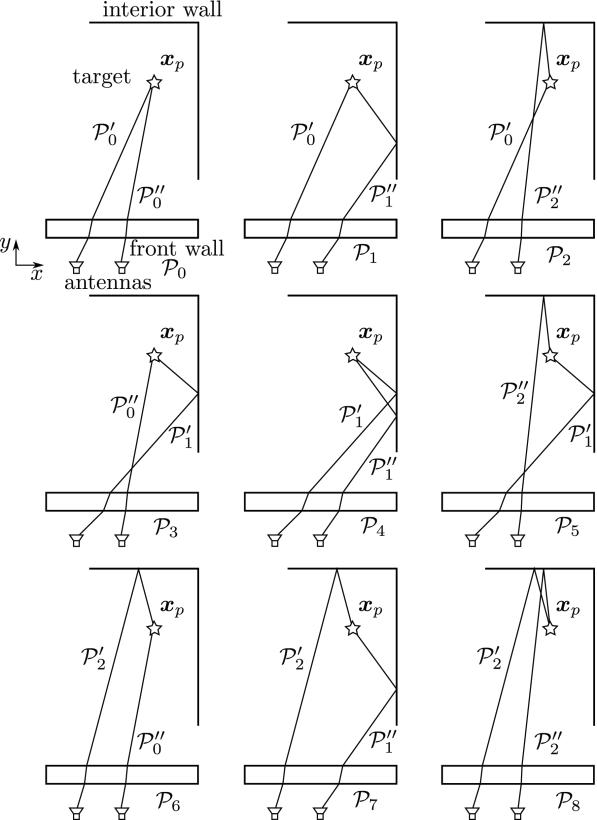
\includegraphics[width=0.5\textwidth]{fig2}
  \caption{CSI处理流程图}
\end{figure}
